\section{Preliminaries}
\label{sec:preliminaries}

\begin{table}[t]
    \centering
   \caption{Frequently used notations.}
   \label{tab:notations}
    \scalebox{0.9}{
        \begin{tabular}{|m{0.26\linewidth}|m{0.74\linewidth}|}
            \hline
            Notation                 & Definition                                                                                       \\
            \hline
            $R$    & a relation or relational table   \\
            \hline
            $\tau$ and $\tau.attr$    & a tuple in a relation, and the value of an attribute of $\tau$ \\
            \hline
            $G(V,E)$         & a property graph with $V$ and $E$                                                          \\
            \hline
            $\pattern(V, E)$   & a pattern graph with $V$ and $E$  \\
            \hline
            $\id(\epsilon)$, $\lab(\epsilon)$, $\epsilon$.attr  & the identifier, label, and the value of given attribute of a graph element $\epsilon$ \\
            \hline
            $\adj(u)$ and $\adj^E(u)$           & neighbors and adjacent edges of $u$           \\
            \hline
            $GR$   & a graph relation     \\
            \hline
            $\matching(GR, \pattern)$, $\matching(\pattern)$  & matching $\pattern$ on a graph relation $GR$ or a graph $G$ \\
            \hline
            $\pi_{A}$, $\sigma_\constraints$, $\Join$  & projection, selection, and join operators over relations \\
            \hline
            $\gproject$, $\gjoin$  & projection and join operators over graph relations \\
            \hline
            $\lambda^s_\lab(e)$, $\lambda^t_\lab(e)$  & the total functions for mapping tuples in an edge relation to source and target vertex relations \\
            \hline
        \end{tabular}
    }
    % \vspace{-.05in}
\end{table}

\revise{In this section, we propose the utilized data model and define the SPJM query processed in this paper. Frequently used notations in this paper are summarized in \reftable{notations}.}

\vspace*{-3mm}
\subsection{Data Model}
\label{sec:data-model}

A schema, denoted as \(S = (a_1, a_2, \ldots, a_n)\), is a collection of attributes. Each attribute \(a_i\) is associated with a specific data domain \(D_i\), which defines the set of permissible values that \(a_i\) can take.
A relation \(R\) is defined as a set of tuples. We consider \(R\) to be a relation over schema \(S\), if and only if, every tuple \(\tau = (d_1, d_2, \ldots, d_n)\) in \(R\) adheres to the schema's constraints, such that the value \(d_i\) for each position in the tuple corresponds to the data domain \(D_i\) of the attribute \(a_i\) in \(S\). In other words, each value \(d_i\) in a tuple \(\tau\) is drawn from the appropriate data domain \(D_i\) for its corresponding attribute \(a_i\).
Moreover, for any tuple \(\tau\) in the relation \(R\), the notation \(\tau.a_i = d_i\) signifies that the attribute \(a_i\) in tuple \(\tau\) has value \(d_i\). 
A table is a representation of a relation with rows corresponds to tuples in the relation, and columns represent attributes in the schema. In this paper, we use the terms of relation and table interchangeably.

We define a \emph{Property Graph} as $G = (V_G, E_G)$,
where $V$ stands for the set of vertices. Let $E \subseteq V \times V$ denote the set of edges in the graph. An edge $e \in E$ is represented as an ordered pair $e = (v_s, v_t)$, where $v_s \in V$ is the source vertex and $v_t \in V$ is the target vertex, indicating that the edge $e$ connects from $v_s$ to $v_t$.
%we use $\id(e)$ and $\lab(e)$ to denote the globally unique id and label of $e$, and $\attr(e, a_i)$, or $e.a_i$, to denote the value of the attribute $a_i$ of $e$.
For any graph element $\epsilon$ that is either a vertex or an edge, we denote $\id(\epsilon)$ and $\lab(\epsilon)$ as the globally unique ID and the label of $\epsilon$, respectively. Given an attribute $a_i$, $\epsilon.a_i$ denotes the value of the attribute $a$ of $\epsilon$.

Given a vertex $v$, we denote its adjacent edges as $\adj_G^E(v) = \{e = (v, v_t) | e \in E\}$ and its adjacent vertices (i.e., neighbors) as $\adj_G(v) = \{v_t | (v, v_t) \in E\}$. It is important to note that the adjacent edges and vertices can be defined for both directions of an edge $e = (v_s, v_t)$, i.e., when $v = v_s$ or $v = v_t$. However, for simplicity, we only define one direction in this notation. In the actual semantics of the paper, both directions may be considered. The degree of $v$ is defined as $d_G(v) = |\adj_G(v)|$, and the average degree of all vertices in the graph is $\overline{d}_G = \frac{1}{|V_G|} \sum_{v \in V_G} d_G(v)$.
In the rest of the paper, when the context is clear, we may remove $G$ from the subscript for simplicity, for example $G=(V, E)$.

Considering two graphs \(G_1\) and \(G_2\), we assert that \(G_2\) is a subgraph of \(G_1\), symbolized as \(G_2 \subseteq G_1\), if and only if \(V_{G_2} \subseteq V_{G_1}\), and \(E_{G_2} \subseteq E_{G_1}\). Furthermore, \(G_2\) qualifies as an induced subgraph of \(G_1\) under the condition that \(G_2\) is already a subgraph of \(G_1\), and for every pair of vertices in \(G_2\), any edge \(e\) that exists between them in \(G_1\) must also present in \(G_2\).

To formalize the integration of graph syntax within the realm of relational data, we introduce the concept of a \textit{Relations-to-Graph Mapping} (i.e. \rgmapping), to facilitate the transformation of relational data structures into a property graph.
%
Specifically, \revise{an \rgmapping comprises a vertex mapping and an edge mapping that maps tuples in relations to unique vertices or edges.
Suppose a tuple $\tau$ in relation $R$ is mapped to a vertex $v \in V$ (or edge $e = (v_s, v_t) \in E$), it is assigned an ID $\id(v)$ (or $\id(e)$) that matches the name of $R$, a label $\lab(v)$ (or~$\lab(e)$), and attributes $v.attr*$ (or $e.attr*$) that mirror the attributes $attr*$ of $\tau$.
Relations mapped to vertices and edges are referred to as vertex relations and edge relations, respectively}.

Given \revise{an edge relation $R_{e}$ and two vertex relations $R_{p_s}$ and $R_{p_t}$, we further define two total functions: $\lambda_{e}^s: R_{e} \to R_{p_s}$ and $\lambda_{e}^t: R_{e} \to R_{p_t}$, which maps a tuple $\tau \in R_{e}$ to a tuple $\tau_s \in R_{p_s}$ and a tuple $\tau_t \in R_{p_t}$, respectively.
Applying the vertex mapping, $\tau_s$ and $\tau_t$ are mapped to the source vertex $v_s$ and target $v_t$ of the edge, respectively.
These total functions are typically established through primary-foreign key relationships, which are best illustrated in an Entity-Relationship (ER) diagram \todo{add a reference for ER-diagram}}.
%For example, an ER diagram is shown in Fig.~\ref{fig:intro-rgmapping-example}(a), and it indicates two total functions w.r.t.~$\relation{\text{Likes}}$, i.e., $\lambda_{\text{Likes}}^s: \relation{\text{Likes}} \to \relation{\text{Person}}$ and $\lambda_{\text{Likes}}^t: \relation{\text{Likes}} \to \relation{\text{Message}}$}.



%\enlargethispage{1em}

%Given two relations, \(R_1\) and \(R_2\), each with its own schema. Let there be a bijective relation mapping, \(\lambda: R_1 \mapsto R_2 \).
\iffalse
\begin{definition}[\rgmapping]
\label{def:rgmapping}
Given two sets of relations $\{R_{p_1}, \ldots,$ $R_{p_n}\}$ and $\{R_{q_1}, \ldots, R_{q_m}\}$,
we define an \rgmapping to map the relations to a property graph $G = (V, E)$, %which contains the mappings of $(\zeta_v, \zeta_e, \lambda_{e_1}^s, \lambda_{e_1}^t, \ldots, \lambda_{e_m}^s, \lambda_{e_m}^t)$,
which are elaborated as follows:

\begin{itemize}
\item \textbf{Vertex Mappings}: $\zeta_v: \bigcup_{i=1}^{n} R_{p_i} \mapsto V$ is a bijective function that maps every tuple $\tau \in R_{p_i}$ for all $1 \leq i \leq n$ to a unique vertex $v \in V$. This vertex $v$ is assigned: an ID $\id(v)$, a label $\lab(v)$ that matches the name of $R_{p_i}$, and attributes $v.attr*$ that mirror the attributes $attr*$ of $\tau$.
The relations that are mapped to vertices in the graph are referred to as vertex relations.

\item \textbf{Edge Mappings}: $\zeta_e: \bigcup_{i=1}^{m} R_{q_i} \mapsto E$ is a bijective function that maps every tuple $\tau \in R_{q_i}$ for all $1 \leq i \leq m$ to a unique edge $e = (v_s, v_t) \in E$. Similar to vertices, each edge $e$ is assigned: an ID $\id(e)$,
a label $\lab(e)$ corresponding to the name of $R_{q_i}$, and attributes $e.attr*$ that reflect the attributes $\tau.attr*$ of $\tau$.
For each edge relation $R_{q_i}$, there are two corresponding vertex relations $R_{p_s}$ and $R_{p_t}$.
We further define two total functions: $\lambda_{q_i}^s: R_{q_i} \to R_{p_s}$ and $\lambda_{q_i}^t: R_{q_i} \to R_{p_t}$, which maps a tuple $\tau \in R_{q_i}$ to a tuple $\tau_s \in R_{p_s}$ and a tuple $\tau_t \in R_{p_t}$, respectively.
The vertices $v_s$ and $v_t$ corresponding to $\tau_s$ and $\tau_t$, respectively, are obtained by applying the vertex mapping function $\zeta_v$, i.e., $v_s = \zeta_v(\tau_s)$ and $v_t = \zeta_v(\tau_t)$.
The relations $R_{q_i}$ that are mapped to edges in the graph are referred to as edge relations.
\end{itemize}
\end{definition}
\fi

\begin{figure*}
    \centering
    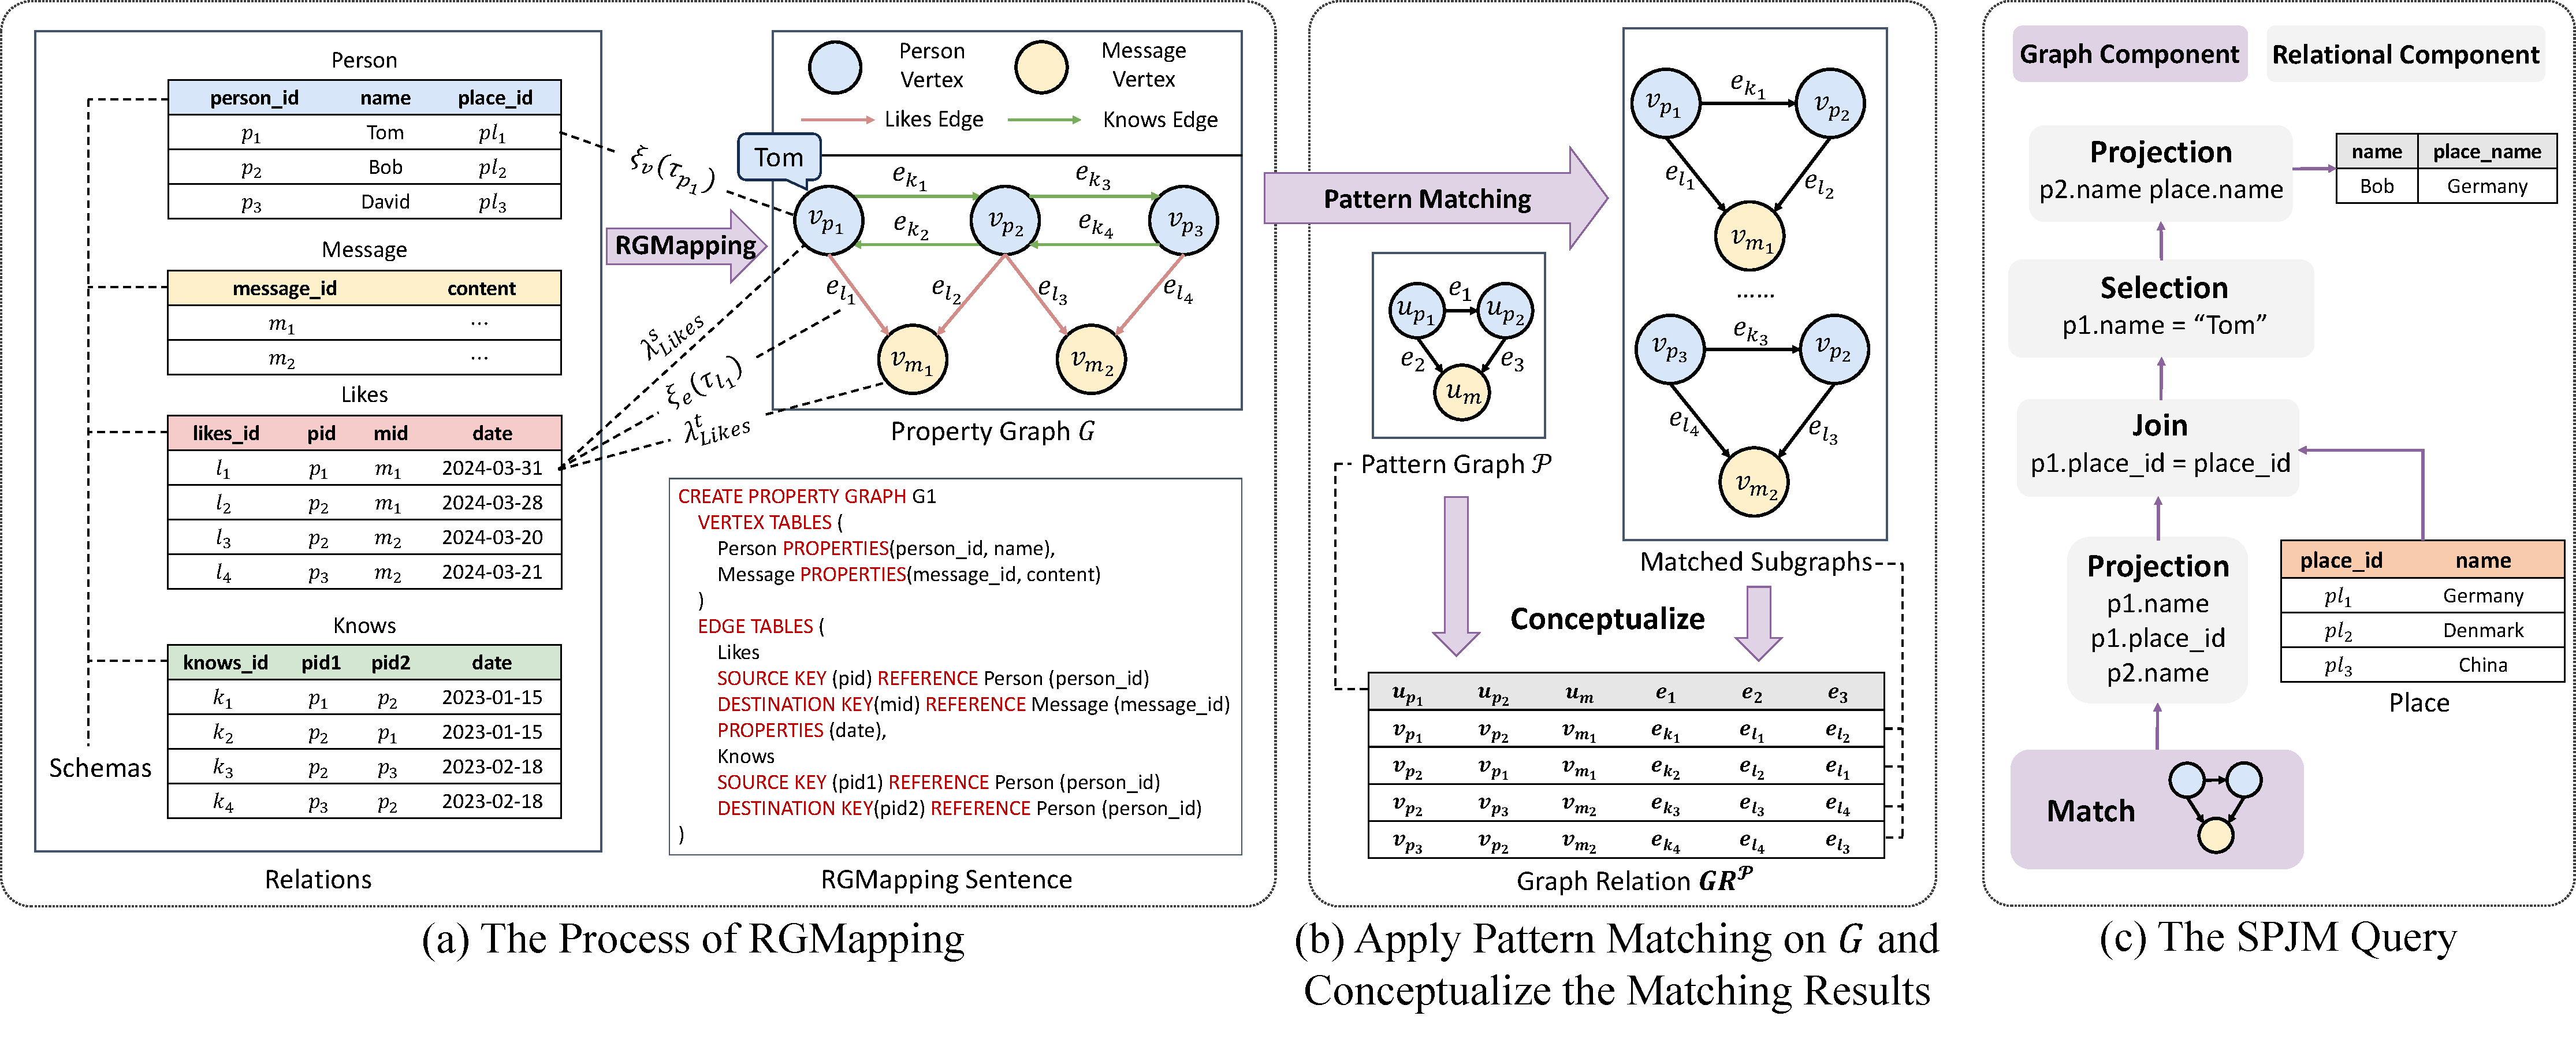
\includegraphics[width=0.95\linewidth]{./figures/rgmapping.pdf}
    \caption{An example of \rgmapping.}
    \label{fig:intro-rgmapping-example}
\end{figure*}

\begin{example}
    \label{ex:rgmapping}
    An \rgmapping can be defined following the grammar of SQL/PGQ with \lstinline{CREATE PROPERTY GRAPH} statements.
    Given the relations, an \rgmapping is defined with the statement shown in Fig.~\ref{fig:intro-rgmapping-example}(a).
    \iffalse
    \begin{equation*}
        \begin{split}
            & \textit{Person = (\underline{person\_id}, name, place\_id)} \\
            & \textit{Message = (\underline{message\_id}, content)} \\
            & \textit{Place = (\underline{place\_id}, pl\_name)} \\
            & \textit{Likes = (\underline{likes\_id}, pid, mid, date)} \\
            & \textit{Knows = (\underline{knows\_id}, pid1, pid2, date)}
        \end{split}
    \end{equation*}
    \fi
    %the following statement defines an \rgmapping (\todo{better plot the statement in Figure 4}):
    \iffalse
    \begin{lstlisting}
CREATE PROPERTY GRAPH G1
    VERTEX TABLES (
       Person PROPERTIES(person_id, name),
       Message PROPERTIES(message_id, content)
    )
    EDGE TABLES (
       Likes
       SOURCE KEY(pid) REFERENCE Person(person_id)
       DESTINATION KEY(mid) REFERENCE Message(message_id)
       PROPERTIES(date),
       Knows
       SOURCE KEY(pid1) REFERENCE Person(person_id)
       DESTINATION KEY(pid2) REFERENCE Person(person_id)
    )
    \end{lstlisting}
    \fi
    The described \rgmapping involves assigning tuples from vertex relations, such as $\relation{Person}$ and $\relation{Message}$, to graph vertices. For instance, the vertex $v_{p_1}$ is associated with the tuple $\tau_{p_1}$ in $\relation{Person}$, and thus assigned the label ``Person'' and the name attribute ``Tom''. Similarly, edge relations $\relation{Likes}$ and $\relation{Knows}$ correspond to graph edges.
    \revise{The ER diagram of the relations are shown in Fig.~\ref{fig:intro-rgmapping-example}(a). Regarding $\relation{Likes}$
    that is mapped to graph edges, two total functions can be identified using the primary-foreign key relationships, namely, $\lambda_{\text{Likes}}^s: \relation{\text{Likes}} \to \relation{\text{Person}}$ and $\lambda_{\text{Likes}}^t: \relation{\text{Likes}} \to \relation{\text{Message}}$.}
    Let's consider the edge $e_{l_1}$. It originates from the tuple $\tau_{l_1}$ in the $\relation{Likes}$ relation. Its source vertex $v_{p_1}$ is linked to the tuple $\tau_{p_1}$ in $\relation{Person}$ via the function $\lambda_{Likes}^s$, following the condition ``$\tau_{l_1}.pid = \tau_{p_1}.\text{person\_id}$''. Similarly, its target vertex $v_{m_1}$ is associated with the tuple $\tau_{m_1}$ in $\relation{Message}$ via the function $\lambda_{Likes}^t$, following the condition ``$\tau_{l_1}.mid = \tau_{m_1}.\text{message\_id}$''. As a result of this mapping, the edge $e_{l_1}$ is assigned the label ``Likes'' and the attribute ``date'' with the value ``2024-03-31''.
\end{example}

%In the rest of this paper, let $\mathcal{J}_{GR} = 2^{2^{V \cup E}}$ be the domain of graph relations, $\mathcal{J}_R = 2^{2^{D}}$ be the domain of relations, and $\mathcal{J} = \mathcal{J}_{GR} \cup \mathcal{J}_R$.

%\enlargethispage{1em}

\vspace*{-3mm}
\subsection{Matching Operator}
\label{sec:matching-operator}
Consider a property graph \(G(V_G, E_G)\), alongside a \emph{connected} pattern graph, represented as \(\pattern(V_\pattern, E_\pattern)\). Here, \(\pattern\) is a property graph that does not possess attributes, and
we denote $n$ and $m$ as the number of vertices and edges in the $\pattern$, respectively.
%Graph pattern matching is defined as the task of identifying all subgraphs within a target graph \(G\) that are \emph{homomorphic} to \(\pattern\).
Graph pattern matching seeks to determine all subgraphs in \(G\) that are \emph{homomorphic} to \(\pattern\).
Formally, given a subgraph $g \subseteq G$, a homomorphism from \(\pattern\) to \(g\) is a \emph{surjective}, total mapping \(f: V_\pattern \cup E_\pattern \to V_{g} \cup E_{g}\) that satisfies the following conditions: (1) For every vertex \(u \in V_\pattern\), there is a corresponding vertex \(v = f(u) \in V_{g}\) with \(\lab(v) = \lab(u)\); (2) For each edge \(e = (u_s, u_t) \in E_\pattern\), there is a corresponding edge \(f(e) = (v_s, v_t) \in E_{g}\), ensuring that the mapping preserves the edge's the label, as well as its source and target vertices, that is \(\lab(e) = \lab(f(e))\), and \(f(u_s) = v_s\), \(f(u_t) = v_t\). It's important to highlight the homomorphism semantics, as one of the widely used semantics for graph pattern matching~\cite{angles2017foundations}, do not require each pattern vertex and edge being uniquely mapped to distinct vertices and edges in the data graph. This facilitates a seamless integration between graph pattern matching and relational operations, but alternative semantics for graph pattern matching such as isomorphism can also be adopted, as will be further discussed in~\refsec{handling-match-operator}.

The outcomes of graph pattern matching can be succinctly modeled as a relation \(GR_G^\pattern\), or more compactly \(GR^\pattern\) in clear contexts, defined over the schema \(S = V_\pattern \cup E_\pattern\). Here, the sets \(V_G\) and \(E_G\) serve as the respective domains for the vertices and edges identified through the matching process. Within this framework, we refer to such a relation as a \emph{Graph Relation}, a construct where all attributes are derived from the domain of a property graph.
It is essential to recognize that any property graph \(G\) can be conceptualized as a graph relation \(GR^G\), represented by a singular tuple that collectively encompasses all of its vertices and edges. Throughout this paper, we treat the notions of a property graph and a tuple of graph relation as essentially interchangeable terms. In alignment with this perspective, we elaborate on the \emph{Matching} operator as follows.

%The formulation of graph relation inherently positions any graph $G$ as a graph relation consisting of a single tuple that encapsulates the entirety of its vertices and edges.
%he results of graph pattern matching can be represented as a relation \(R_G(\pattern)\) (or \(GR(\pattern)\) for short when the context is clear) over the schema  \(S = V_\pattern \cup E_\pattern\), wherein \(V_G\) and \(E_G\) act as the domains for the vertices and edges that have been matched, respectively. In this paper, we call such a relation a \emph{graph relation}, when all attributes of the relation are from the domain of a property graph.
%It's clear that any graph $G$ can be represented as a graph relation consisting of a single tuple that encapsulates the entirety of its vertices and edges. In this paper, the concepts of property graph and graph relation can always be used interchangeably. In this context, we introduce the \emph{Match} operator as detailed below.

%likewise expressible as a graph relation \(GR_G(\pattern)\) (or \(GR(\pattern)\) for short when the context is clear) based on the schema \(S = V_\pattern \cup E_\pattern\), wherein \(V_G\) and \(E_G\) act as the domains for the vertices and edges that have been matched, respectively. In this context, we introduce the \emph{Match} operator as detailed below.

\begin{definition}[Matching Operator, \(\matching\)]
    \label{def:matching}
    The Matching Operator, denoted as \(\matching\), is designed to perform graph pattern matching on a given graph relation \(GR\) against a specified pattern graph \(\pattern\). For each graph instance \(g\) in \(GR\), \(\matching\) identifies all subgraphs of \(g\) that are homomorphic to \(\pattern\), and subsequently, aggregates these mappings to construct a comprehensive graph relation. The operation of the matching Operator can be formally articulated as \(\matching(GR, \pattern) = \bigcup_{g \in GR} GR_g^\pattern\).%, where each \(GR_g^\pattern\) represents the subgraph(s) of \(g\) that align with the structure and properties of \(\pattern\).
\end{definition}

\begin{example}
    \label{ex:matching}
    Let \(G\) denote the property graph derived from the relations via \rgmapping in \refex{rgmapping}.
    Given a pattern graph \(\pattern\) in \reffig{intro-rgmapping-example}(b), the results of graph pattern matching are subgraphs of \(G\) that are homomorphic to \(\pattern\), represented as a graph relation \(GR^\pattern = \matching(GR^{G}, \pattern)\), each tuple corresponds to one matched subgraph.
\end{example}

This definition ensures that the matching operator is inherently closed regarding graph relations,
which adheres to the language opportunities of ``nested matching'' (specified as PGQ-079) in SQL/PGQ~\cite{sql-pgq}.
In this paper, we only handle cases where $G$ represents the entire property graph, and thereafter simplify the matching operator notation to $\matching(\pattern)$ when the context is clear.

%\enlargethispage{1em}

\vspace*{-1mm}
\subsection{Problem Definition}
\label{sec:problem-definition}

To study relational query optimization, it is common to focus on a category of queries known as \spj queries,
which encapsulate the three most frequently employed operations in database management: select, project, and (natural) join.
These operations form the backbone of many relational queries. Given a set of relations \(R_1, R_2, \ldots, R_m\),
an \spj query is formally represented as:
\[
Q = \pi_A(\sigma_\constraints(R_1 \Join \cdots \Join R_m)).
\]

Inspired from the \spj paradigm, we introduce a novel category of queries, termed \spjm queries, to logically formulate SQL/PGQ~\cite{sql-pgq} queries that
blend relational and graph operations. Our focus is not on an exhaustive exploration of SQL/PGQ, which encompasses a broad spectrum of operations such as shortest-path, but rather on understanding and enhancing the core functional elements of such queries.
The \spjm framework augments \spj queries by incorporating a matching operator, thereby enriching the query's expressive power to seamlessly navigate both relational and graph data domains.
Given the set of relations and a property graph \(G\) constructed from these relations via an \rgmapping, %(\refdef{rgmapping}),
an \spjm query is articulated as:
\begin{equation}
    \label{eq:spjm}
Q = \pi_A(\sigma_\constraints(R_1 \Join \cdots \Join R_m \Join (\widehat{\pi}_{A*}\matching_G(\pattern))))
\end{equation}
In this formulation, \(\widehat{\pi}_{A*}\matching_G(\pattern)\) is the \emph{graph component} of
the query, while the remaining part of the query is an \spj expression referred to as the \emph{relational component}.
Here, \(\matching_G(\pattern)\) represents the process of matching the pattern \(\pattern\) on the graph \(G\) and
returns a graph relation as defined in \refdef{matching}. The operator \(\widehat{\pi}_{A*}\) is a
graph-calibrated projection operator that extracts the ID, label, and other attributes from the vertices and edges in the matched results.
This process helps ``flatten'' graph elements into relational tuples.
For example, given a graph relation $GR$ that contains a vertex of \{ID:0, label:Person, name:``Tom''\}, the
following projection
\[
\widehat{\pi}_{\id(v) \rightarrow \text{v\_id}, \lab(v) \rightarrow \text{v\_label}, v.name \rightarrow \text{v\_name}}(GR)
\]
turns the vertex into a relational tuple of (0, Person, ``Tom'').
The projection operation is designed to reflect the \lstinline{COLUMNS} clause in SQL/PGQ
to retrieve specific attributes from vertices and edges as required. For simplicity, we assume that all
attributes are extracted unless otherwise specified.

In this paper, we study the problem of optimizing \spjm queries in \refeq{spjm}. \reffig{intro-rgmapping-example}(c) illustrates the \spjm query skeleton corresponding to the SQL/PGQ query in \refex{introduction:sqlpgq}.

\comment{
\begin{example}
    \reffig{intro-rgmapping-example}(c) illustrates an example of an \spjm query, along with its corresponding SQL/PGQ expression. The query's semantic is to identify Tom's friends (and their living place) who like the same messages as Tom. As per the query, once the results of the matching operator are obtained (as described in \refex{matching}), a $\gproject$ operator is applied to extract attributes from all vertices, forming a relational table. Subsequently, the join, selection, and projection operators are employed to compute the final results.
    %Specifically, Tom, who is German, and Bob know each other and like the same message $m_1$.
\end{example}
}

%is a relation generated by projecting the outputs of the matching operator $\mathcal{M}$ to relations of properties.
%Besides, $GR_i$ is the graph relation that contains the data graphs that pattern matching is conducted on and $\mathcal{P}_i$ is the pattern.
%$prop_i$ is a list of necessary properties of vertices and edges in the resultant relation.

\iffalse
Regarding the SPJM problem, the main difference between the aforementioned four types of optimizers lies in their search space when optimizing the physical implementation of the matching operator.
Specifically, for $Rel$ methods, the matching operator is implemented with only joins that do not leverage graph indices (named relational joins) such as hash joins.
Therefore, $\widetilde{R}_i$ can be optimized with the relational optimizer.
For $Rel^+$ methods, in the process of optimization, the matching operator is implemented with relational joins.
Thus, the relational optimizer is also utilized to optimize $\widetilde{R_i}$.
However, after that, relational joins are replaced with joins that leverage graph indices (named graph joins) if possible such as sip join in GRainDB.
For $Rel+G$ methods, graph joins are considered in implementing the matching operator.
Then, operators inside of $\widetilde{R}_i$ are optimized by the graph optimizer, while the operators out of $\widetilde{R}_i$ are optimized by the relational optimizer.
Besides, the optimizations cannot be simultaneously related to operators within and outside of $\widetilde{R}_i$.
For example, the filter operators, i.e., $\sigma_d$ cannot be pushed into $\widetilde{R}_i$.
For $Rel\&G$, such optimizations are allowed.
\fi

% The search space for relgo in the context of a SPJG query consists of operator trees that correspond to sequence of join operators, e.g., the sequence
% \begin{lstlisting}
%     Join(Join(Join(Join(GR_1, GR_2), R_1), R_2), R_3)
% \end{lstlisting}


\iffalse
\subsection{Equivalence Between Graph Pattern Matching and Graph Relational Operators}
\label{sec:proof-gpm-gro}

For the SPJG problem to be solved in this paper, we need to obtain the graph relations by pattern matching.
In detail, the pattern matching process ought to be expressible through the traversal of paths, which are sequences of source, expand, and join operators.
In this section, we prove that the matching operator can be replaced with source, expand, and join operators. without changing the semantics of the query.
Then, the matching order can be further optimized by relgo.

We start from the case that there is only one path in the specified pattern, and firstly, we focus on homomorphic pattern matching.
Then, we have the following theorem.

\begin{theorem}
    Homomorphic pattern matching with a path pattern can be expressed with graph relational algebra expressions.
\end{theorem}
\begin{proof}
    The graph relational algebra operators related to pattern matching include source, expand, join, and extend-intersect.
    Then, we prove the theorem by induction.
    Let each vertex and edge in a path pattern be an element.
    If for each edge in a pattern, its adjacent vertices are also specified in the pattern, then the pattern is called a strict pattern $P$.
    Otherwise, it is a loose pattern $\hat{P}$.

    %Since path patterns specified in SQL/PGQ are all strict patterns are, the induction is conducted on the number of elements in the strict pattern.
    The path pattern is a strict pattern, and induction is conducted on the number of elements in the strict pattern.
    When there is only one element (i.e., a vertex like ``(u:Label)'') in the pattern, the corresponding algebra expression of the pattern is $\bigcirc_{(u:\text{Label})}$, and it is clear that the expression equals the pattern.

    Then, suppose for a path pattern with at most $n$ elements, the corresponding algebra expressions have the same meaning as matching the path pattern.
    Denote a graph relational algebra with the same meaning as matching path pattern $P$ by $E_p$.

    When there are $n + 1$ elements in the path pattern $P$:

    %Condition 1: $P = P_1, P_2$, i.e., pattern $P$ is obtained by concatenating subpatterns $P_1$ and $P_2$.
    %(e.g., $P_1 = (u)-[e]-(v), P_2 = (u)-[e']-(w), P = (u)-[e]-(v), (u)-[e']-(w)$).
    %Then, $E_{p_1} \Join E_{p_2}$ equals $P$, since join operator implemented in relational databases follows the semantics of homomorphism.


    Condition 1: $P = P_1 - \hat{P}_2$.
    Without loss of generality, suppose vertex $v$ in $P_1$ is adjacent to an edge in $P_2$.
    (e.g., $P_1 = (u)-[e]-(v), P_2 = [e']-(w), P = (u)-[e]-(v)-[e']-(w)$).
    Then, let $P_3 = (v)-\hat{P}_2$, and the corresponding algebra expression of $P$ can be $E_{p_1} \Join E_{p_3}$.
    $E_{p_1} \Join E_{p_3}$ equals $P$, since join operator implemented in relational databases follows the semantics of homomorphism.
    Moreover, if $\hat{P}_2$ only consists of one vertex and an edge adjacent to it (i.e., $\hat{P}_2 = [e:eLabel]-(v_t:vLabel)$).
    Then, the corresponding algebra expression of $P$ can also be $\updownarrow_{(v)}^{(v_t:vLabel)}[e:eLabel]E_{p_1}$.
    The expand operator is also implemented by joining relational tables, which follows the semantics of homomorphism.

    Condition 2: $P = P_1$ extends $v$ through edges $[e_1:eLabel1], \cdots [e_k:eLabelk]$ ($k \geq 1$), i.e., at least one vertex in $P_1$ connects to vertex $v$.
    Then, the corresponding algebra expression of $P$ is
    \begin{equation*}
        E_{p_1} \Diamond_{v_1, \cdots, v_k}^{eLabel1, \cdots, eLabelk} \bigcirc_{(v:vLabel)}.
    \end{equation*}
    Since the extend-intersect operator is implemented with relational joins and follows the semantics of homomorphism, the algebra expression has the same meaning as matching the path pattern.

    In conclusion, the corresponding algebra expressions of path pattern $P$ with $n + 1$ elements have the same meaning as matching the path pattern.

    In conclusion, adopting the homomorphism semantics, matching path patterns has the same meaning as the corresponding graph relational algebra expressions.
\end{proof}

When the match operator adopt the isomorphic semantics, it is straightforward to add some constraints with selection operators to get the graph relational expressions equal to the match operator.
Furthermore, when there are more than one path specified in the pattern, the expressions for different paths can be connected with join operators and the obtained expressions equal to the match operator.


Besides the WALK mode by default, when the path patterns are in TRAIL, ACYCLIC, or SIMPLE mode, we still have the same conclusions.
Specifically, in TRAIL, ACYCLIC, or SIMPLE mode, a selection operator needs to be added to remove the results with repeated edges or vertices.
In detail, the selection operator should wrap the corresponding algebra expression of path patterns in the WALK mode.
For example, in the TRAIL mode, the corresponding graph relational algebra expression of $P = P_1 - P_2$ is $\sigma_{c}(E_{p_1} \Join E_{p_2})$ or $\sigma_{c}(\updownarrow_{(v)}^{(v_t:vLabel)}[e:eLabel]E_{p_1})$, where $c$ is the condition specifying that every two different pattern edges bind to different edges in each result.
In the ACYCLIC and SIMPLE mode, condition $c$ should be specified according to the constraints of the mode.

Furthermore, there may be more than one path patterns specified in the <Pattern> part of SQL/PGQ queries, and the different path patterns may have different path modes.
Denote the path patterns by $P_1, \cdots, P_k$.
According to SQL/PGQ, the binding results of different path patterns are joined together.
If the match mode in SQL/PGQ is set to \textbf{REPEATABLE ELEMENTS}, there is no more constraint, and ``MATCH $P_1, \cdots, P_k$'' has the same meaning as $P_1 \Join \cdots \Join P_k$, both of which have the semantics of homomorphism.
Otherwise, if the match mode in SQL/PGQ is set to \textbf{DIFFERENT EDGES}, the same edge cannot bind to different variables in different path patterns.
Therefore, a selection operator is needed, and ``MATCH $P_1, \cdots, P_k$'' has the same meaning as $\sigma_{d}(P_1 \Join \cdots \Join P_k)$, where $d$ is the condition specifying that each edge cannot bind to more than one variables across all path patterns.
\fi
